\documentclass[10pt, xcolor=x11names,compress]{beamer}
\usepackage{tabulary}
\usepackage{booktabs}
\usepackage{float}
\usepackage{graphicx}
\usepackage{mwe}% for example pictures
\usepackage{siunitx}
\usepackage{hyperref}
\usepackage{amsmath}
\usepackage{caption}
\usepackage{tikz}
\usetikzlibrary{arrows.meta, positioning, shadows.blur}
\usetikzlibrary{shapes}
\usepackage{fontawesome5}

\usecolortheme{spruce}
\useoutertheme{infolines}
\usefonttheme[onlymath]{serif}
\setbeamertemplate{headline}[default]
\setbeamertemplate{navigation symbols}{}
\mode<beamer>{\setbeamertemplate{blocks}[rounded][shadow=true]}
\setbeamercovered{transparent}
\setbeamercolor{block body}{use=structure, fg=white, bg=black!20}
\setbeamercolor{itemize item}{fg=black}
\setbeamercolor{itemize subitem}{fg=gray} 
\setbeamercolor{itemize subsubitem}{fg=black!20} 
\makeatletter\setbeamertemplate{footline}
{  
\leavevmode%  
\hbox{%  
\begin{beamercolorbox}[wd=.333333\paperwidth,ht=2.25ex,dp=1ex,center]{author in head/foot}%    
\usebeamerfont{author in head/foot}
\insertshortauthor%~~\beamer@ifempty{\insertshortinstitute}{}
 \end{beamercolorbox}%  
 \begin{beamercolorbox}[wd=.333333\paperwidth,ht=2.25ex,dp=1ex,center]{institute in head/foot}%    
 \usebeamerfont{title in head/foot}\textbf{AREC 615 Project} 
 \end{beamercolorbox}%  
 \begin{beamercolorbox}[wd=.333333\paperwidth,ht=2.25ex,dp=1ex,right]{date in head/foot}%    
 \usebeamerfont{date in head/foot}\insertshortdate{}\hspace*{2em}    
 \insertframenumber{} / \inserttotalframenumber\hspace*{2ex}   
 \end{beamercolorbox}}%  
 \vskip0pt%
 }
 \makeatother 
 \useoutertheme[footline=empty, subsection=false]{miniframes}
 \usepackage{multicol}  
 \author{Sushil Khatri}
 \title{\textbf{AREC 615 Project}\\ Agricultural Productivity and Soil Carbon Dynamics: A Bioeconomic Model}

 \institute{Department of Agricultural and Resource Economics \\ Colorado State University}
 \date{Dec 04, 2025} 
 \begin{document}
 \begin{frame}
 \titlepage
 \end{frame}

 \begin{frame}{Table of Contents}
    \tableofcontents
\end{frame}

\section{Introduction}
\subsection{Paper Information}
\begin{frame}[label=Paper Information]{Paper Information}
\begin{itemize}
    \item \textbf{Paper Title:} Agricultural Productivity and Soil Carbon Dynamics: A Bioeconomic Model
    \item \textbf{Authors:} J. Berazneva, J. M. Conrad, D. T. Güereña, J. Lehmann, and D. Woolf
    \item \textbf{Journal:} American Journal of Agricultural Economics (AJAE)
    \item \textbf{Year:} 2019
\end{itemize}
\end{frame}



\subsection{Problem}
\begin{frame}[label=Problem]{Problem}
\centering

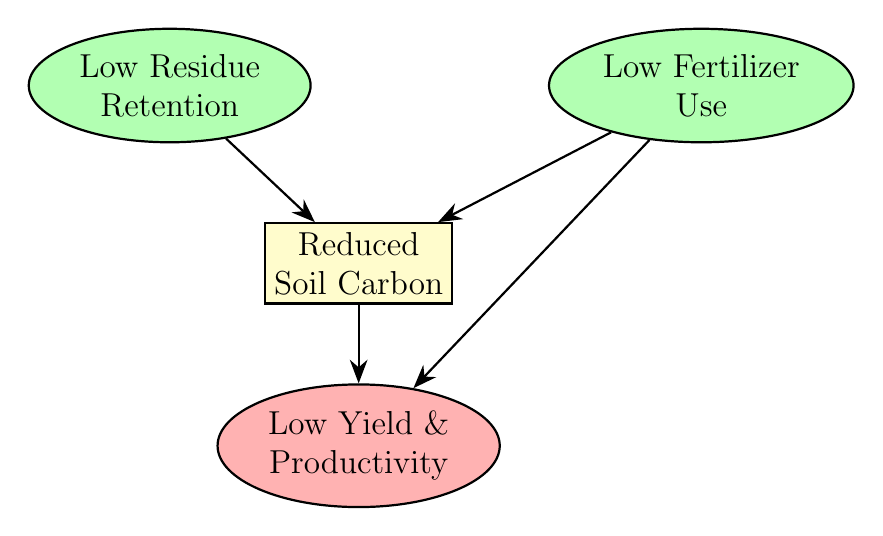
\begin{tikzpicture}[
    node distance=1cm,
    every node/.style={font=\large},
    ovalnode/.style={
        ellipse,
        draw=black,
        thick,
        minimum width=1cm,
        minimum height=1cm,
        align=center
    },
    rectnode/.style={
        rectangle,
        draw=black,
        thick,
        minimum width=1cm,
        minimum height=1cm,
        align=center
    }  
]


\node[ovalnode, fill=green!30, xshift=-1cm] (residue) 
    {Low Residue\\Retention};
\node[ovalnode, fill=green!30, right=3cm of residue] (fertilizer) 
    {Low Fertilizer\\Use};
\node[rectnode, fill=yellow!20, below=1cm of residue, xshift=2.4cm]
    (soil) {Reduced\\Soil Carbon};
\node[ovalnode, fill=red!30, below=1cm of soil]
    (yield) {Low Yield \&\\Productivity};


\draw[-{Stealth[length=3mm]}, thick, black!70!black] (residue) -- (soil);
\draw[-{Stealth[length=3mm]}, thick, black!70!black] (fertilizer) -- (soil);
\draw[-{Stealth[length=3mm]}, thick, black!70!black] (soil) -- (yield);
\draw[-{Stealth[length=3mm]}, thick, black!70!black] (fertilizer) -- (yield);

\end{tikzpicture}

\vspace{0.5cm}

\only<2->{
\textbf{Research Question:}  
\textit{What fertilizer–residue choices maximize long-run soil carbon and yield?}
}
\end{frame}


\subsection{Model Components}
\begin{frame}[label= Model Components]{Model Components}

\textbf{Control Variables}
\begin{itemize}
    \item $f_t$ : fertilizer applied (Mg/ha)
    \item $a_t$ : fraction of crop residue retained (0–1)
\end{itemize}

\textbf{State Variable}
\begin{itemize}
    \item $c_t$ : soil organic carbon stock (Mg/ha)
\end{itemize}


\textbf{Yield Function}

\[
\begin{aligned}
y_{kit}
&= \alpha_0 
+ \alpha_c \, c_{kit}
+ \alpha_{cc} \, c_{kit}^2
+ \alpha_f \, f_{kit}
+ \alpha_{ff} \, f_{kit}^2
+ \alpha_{cf} \, c_{kit} f_{kit} \\[6pt]
&\quad 
+ \textcolor{blue}{
\underbrace{\gamma_k + \phi_i + \eta_t + \nu_{kt}}_{\text{Fixed Effects}}
}
+ \kappa_{kit}
\end{aligned}
\]

\textbf{Soil Carbon Dynamics}
\[
c_{t+1} = c_t -D c_t + 
A \left(a_t F k \, y(c_t,f_t)\right)^B
\]

\begin{itemize}
    \item $D$ : annual SOC decay rate  
    \item $A, B$ : accumulation parameters (soil science models)
    \item $F$ : residue carbon fraction  
    \item $k$ : residue-grain ratio \hyperlink{Replication}{\beamergotobutton{Replication}}
\end{itemize}
\end{frame}


\subsection{Optimization Structure}
\begin{frame}[label= Optimization Structure]{Optimization Structure}
\textbf{Objective Function}
\[
\begin{aligned}
\max_{\{f_t, a_t\}} \quad 
& \sum_{t=0}^{\infty} \beta^t \, \pi(c_t, f_t, a_t) \\
\text{s.t.} \quad 
& c_{t+1} = c_t - D c_t + 
A \left(a_t F k \, y(c_t, f_t)\right)^B 
\end{aligned}
\]

\textbf{Profit Function}
\[
\pi(c_t, f_t, a_t)
=
\bigl( p_{maize}
      + q_R \, k_{rg} \, (1 - a_t) \bigr)
\, y(c_t, f_t)
\;-\; nP \, f_t
\;-\; m_{fix} .
\]

\end{frame}




\section{Results}
\begin{frame}[label= Results]{Results}

\textbf{Steady-State Optimal Values}
\[
f^{*} = 0.13 \quad \text{Mg/ha}
\]
\[
a^{*} = 0.54 \quad \text{(54\% residue retention)}
\]
\[
c^{*} = 25.63 \quad \text{Mg C/ha}
\]

\textbf{Optimal Yield}

\[
y^* \approx 3.9 \;\text{Mg/ha}
\]

\textbf{Shadow Value of Soil Carbon}
\[
\lambda^* \in [95,168]\;\$/\text{Mg C}
\]

\end{frame}

\section{Replication}
\begin{frame}[label= Replication]{Replication}

\textbf{Built model}
\begin{itemize}
    \item Set horizon ($T=100$)
    \item Paper consistent discounting, prices, costs, and parameters were used.
    \item Adjusted intercept $b_0$ to match the paper’s steady-state yield.
\end{itemize}

\vspace{0.4cm}
\textbf{Soil Carbon Dynamics}
\begin{itemize}
    \item Calibrated $A$ so paper’s steady state $(c^*,f^*,a^*)$ satisfies the equation.
    \hyperlink{Model Components}{\beamergotobutton{Back to Model}}
\end{itemize}

\vspace{0.4cm}
\textbf{Open-loop Optimization}
\begin{itemize}
    \item Decision vector: $x = [f_1..f_{100}, a_1..a_{100}]$.
    \item Used L-BFGS-B to maximize present value of profits.
    \item Added terminal and tail penalties to enforce convergence.
\end{itemize}
\end{frame}


\subsection{Simulation Results}
\begin{frame}[label= Simulation Results]{Simulation Results}
\begin{figure}
    \centering
    \includegraphics[width=0.8\textwidth, height=0.7\textheight]{100 years.jpeg}
    \caption{Soil carbon, Yield, Fertilizer (Nitrogen), and Residue paths (replication)}
\end{figure}

\end{frame}

\section{Extension}
\begin{frame}
     \begin{center}
        {\Huge \textbf{Extension}} \\
        \rule{0.5\linewidth}{0.7pt} % horizontal line
    \end{center}
\end{frame}


\subsection{Motivation}
\begin{frame}[label=Motivation]{Motivation}
\begin{itemize}
\item \textbf{The original model assumes:} 
\begin{itemize}
    \item No policy intervention
    \item Does not explore how carbon subsidies affect human behavior.
\end{itemize}

    \vspace{1cm}
    \only<2->{
\item \textbf{Extension Idea (flow Subsidy):} 
\begin{itemize}
        \item The government pays a subsidy for annual gains in soil carbon.
    \end{itemize}
    }
    
    \vspace{1cm}
    \only<3->{
    \item \textbf{Key questions for extension:} 
    \begin{itemize}
        \item \textbf{RQ 1:} How do carbon incentives (i.e., \$ per Mg of carbon gained) affect decisions?

        \item \textbf{RQ 2:} How do carbon subsidies affect overall welfare and carbon gain?
    \end{itemize}
    }
\end{itemize}
\end{frame}


\subsection{Extension Model}
\begin{frame}[label=Extension Model]{Extension Model}

\textbf{Carbon-Flow Subsidy Term}
\[
\text{Subsidy}_t = p_C \, (c_{t+1} - c_t)
\]

$p_C$ : carbon payment (\$/Mg of SOC increase)


\vspace{0.5cm}

\textbf{New Profit Function}
\[
\pi^{new}(c_t, f_t, a_t) 
= \pi(c_t, f_t, a_t) 
+ \textcolor{blue}{p_C (c_{t+1} - c_t)}
\]

\vspace{0.4cm}

\textbf{New Objective Function}
\[
\sum_{t=0}^{T} 
\beta^{t} 
\left[
\pi(c_t,f_t,a_t) + \textcolor{blue}{p_C (c_{t+1} - c_t)}
\right]
\]
\end{frame}

\section{Results}
\subsection{Extension Results: Optimal behavior}
\begin{frame}[label=Extension Results]{RQ 1 Extension Results}

\begin{table}[h!]
\centering
\scriptsize
\captionsetup{justification=raggedright, singlelinecheck=false}
\caption{Effect of Carbon Incentives on Optimal Decisions}
\resizebox{\textwidth}{!}{
\begin{tabular}{c c c c}
\toprule
Carbon price (\$) & Tail residue  \footnotemark[1] & Tail fertilizer \footnotemark[2](Mg N/ha)  & Soil Carbon (Mg/ha) \\
\midrule
0   & 0.54 & 0.13 & 25.60 \\
50  & 0.56 & 0.13 & 26.41 \\
100 & 0.60 & 0.13 & 27.69 \\
150 & 0.78 & 0.11 & 31.49 \\
200 & 0.78 & 0.11 & 31.60 \\
\bottomrule
\end{tabular}
}
\end{table}
\footnotetext[1]{Average residue retention in final 10 years}
\footnotetext[2]{Average fertilizer use in final 10 years}
\end{frame}


\subsection{Extension Results: Welfare Gain}
\begin{frame}{RQ2: Welfare and yield gain}

\begin{figure}
    \centering
    \includegraphics[width=0.8\textwidth, height=0.7\textheight]{Rplot02.jpeg}
    \caption{Welfare and Yied gain}
\end{figure}

\end{frame}

\subsection{Extension Results: Carbon gains}
\begin{frame}{RQ2: Carbon gain}

\begin{figure}
    \centering
    \includegraphics[width=0.8\textwidth, height=0.7\textheight]{Rplot03.jpeg}
    \caption{Soil Carbon Gain and CO$_2$e Response}
\end{figure}

\end{frame}


\section{Conclusion}
\subsection{Conclusion}
\begin{frame}[label=Conclusion]{Conclusion}
\begin{itemize}
    \item Carbon incentives increase residue retention and soil carbon in the long run.
    \item The higher the carbon price, the greater the SOC gains and welfare improvements.
    \item Therefore, carbon payment can increase profitability and promote sustainable agriculture.
\end{itemize}
\end{frame}

\begin{frame}
 \begin{center}
{\Huge \textbf{Thank You!}}\\[0.8cm]
{\Large Questions?}\\[0.4cm]
{\large \faGithub\ \textcolor{blue}{\url{https://github.com/khatris04/AREC-615-Project}}}
	\end{center}
\end{frame}

\end{document}